\mysection{Pedestrian Tracking: KTH Dataset [2]}

\vspace{1\baselineskip}

\begin{minipage}[c]{0.45\textwidth}
    \centering
    \vspace{-1.5em}
    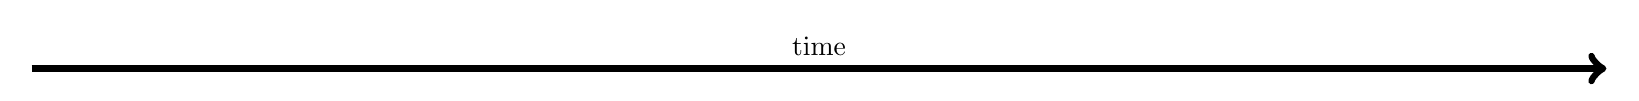
\begin{tikzpicture}
    \draw[line width=1mm, ->] (-10, 0) -- node[above] {time} (10, 0);
    \end{tikzpicture}
    \includegraphics[width=\textwidth]{kth_overlay_16}
    
    \begin{minipage}[c]{0.55\textwidth}
        \begin{itemize}
            \item Attention, prediction and ground-truth overlap at initialization.
            \item Every $16^{th}$ frame of the\\ sequence at 25 fps.
            \item $2^{nd}$ row: attention glimpses multiplied with appearance attention.
        \end{itemize}
    \end{minipage}\hfill   
    {\Large
    \begin{minipage}[c]{0.45\textwidth}
    	\hspace{.9em}
        \begin{tabular}{c|c}
            \multicolumn{2}{c}{Intersection over Union}\\
            Kahou \emph{et. al.} [1] & Ours\\
            \midrule
            0.55 & \B{0.77}
        \end{tabular}
    \end{minipage}
}
    \vspace{.5em}
\end{minipage}

